\chapter{Taxonomie de la co-simulation}\label{sec:tax}
\section*{Introduction}
Les systèmes d'ingénierie intègrent de multiples éléments dans un processus complexe, comprenant des composants physiques, des logiciels et leurs interactions. Cette complexité pose de nombreux défis pour la modélisation et pour la simulation de ces systèmes. L'une des façons de simuler des systèmes comprenant plusieurs composants consiste à modéliser et à simuler l'ensemble du système à l'aide d'un seul outil, ce que l'on appelle la simulation monolithique. L'autre approche consiste à simuler le système dans le cadre d'une co-simulation. 

La co-simulation se définit comme le couplage d'au moins deux unités de simulation distinctes. Ces unités peuvent différer par l'outil de simulation employé, l'algorithme de résolution mis en œuvre, ou encore le pas de temps de résolution utilisé. Une unité de simulation, quant à elle, représente une entité logicielle exécutable responsable de la simulation d'une partie spécifique du système \cite{1,2}. Cette approche présente un potentiel considérable et a été exploitée dans divers domaines, notamment l'industrie automobile \cite{b1}, la gestion de l'électricité \cite{b2}, le chauffage, la ventilation et la climatisation (HVAC) \cite{b3}, le domaine maritime \cite{b4}, et la robotique \cite{b5}.

Dans ce chapitre, on entreprend une révision de l'état de l'art de la co-simulation, en mettant l'accent sur le standard FMI. Notre contribution réside dans la proposition d'une nouvelle approche pour la taxonomie de la co-simulation, visant à décomposer et à simplifier l'analyse de l'état de l'art en détaillant ses fonctionnalités, les exigences et les contraintes de la co-simulation. Cette approche permet une meilleure compréhension des tenants et aboutissants de la co-simulation, ouvrant ainsi la voie à de nouvelles avancées dans ce domaine.

Dans la section \ref{sec:2}, on effectue une présentation et une critique de l'existant en introduisant le standard FMI dans le cadre de la co-simulation, la section \ref{sec:3} présente le processus d'orchestration des scénarios de co-simulation et ses contraintes. La section \ref{sec:4} contient les résultats de l'étude taxonomique menée.


\section{Le standard FMI et la co-simulation}\label{sec:2}
\subsection{FMI}
FMI (Functional Mock-up Interface) \cite{b6}, est un standard élaboré dans le but de créer une interface unifiée pour l'exécution de modèles de systèmes dynamiques, facilitant ainsi l'interopérabilité entre les outils de modélisation et de simulation. L'essence de ce standard réside dans la génération et l'échange de modèles conformes à la spécification FMI entre différents outils. Ces modèles sont, selon le standard, des FMUs (Functional Mock-up Units). 
On distingue deux modes d'utilisation principaux : l'échange de modèle (ME), où le modèle, dépourvu de solveur intégré, requiert la prise en charge de la résolution par l'utilisateur, et la co-simulation (CS), où les modèles sont exportés avec un solveur de l'outil d'import.

L'idée fondamentale derrière le FMI est de permettre aux utilisateurs de combiner des modèles provenant de divers environnements de développement et de simulation, sans être enchaînés par les restrictions d'un outil particulier. En d'autres termes, les FMUs encapsulent les modèles dans une structure standardisée, ce qui permet à ces modèles d'être facilement intégrés dans un environnement de co-simulation, où ils peuvent interagir de manière cohérente avec d'autres composants du système. Cette approche favorise la réutilisation des modèles, réduisant ainsi les efforts de développement et améliorant l'efficacité de la modélisation et de la simulation dans divers domaines d'application.

Dans le cas de la co-simulation, le standard décrit une interface discrète du modèle dynamique, par exemple, étant donnés l'état interne à l'instant $t_n$, les entrées $u_n$, le pas de communication de la co-simulation $h$, $p$ les paramètres fournis, et $y_{n+1}$ le vecteurs des sorties à l'instant $t_{n+1}= t_n + h$ peut être noté comme suit: 
\begin{equation}
    y_{n+1} = \psi_p (u_n,h)
\end{equation}

L'évolution de l'état et du temps est latente, et n'est pas décrite par le standard. Ainsi, les événements sont traités en interne. En plus, l'accès à l'état n'est possible\footnote{Pour la version 2.0.x du standard, pourtant la version 3.x offre la possibilité d'accès à tout instant t} qu'aux points de communication $n\cdot h$.

\subsection{La co-simulation }
Malgré l'intérêt grandissant pour les bénéfices et les défis scientifiques de la co-simulation, ainsi que la diversité des outils disponibles, il est à noter qu'aucune étude connue n'a encore entrepris une analyse comparative approfondie des différentes plateformes de co-simulation et de leurs limitations.

Dans l'article \cite{b7}, Gomes et al. réalisent une revue de la littérature technique portant sur les divers algorithmes développés, en segmentant la co-simulation en trois grandes catégories :
\begin{enumerate}
  \item DE : Co-simulation basée sur des événements discrets.
  \item CT : Co-simulation basée sur le temps continu.
  \item Hybride : Approche hybride de la co-simulation.
\end{enumerate}

Ils présentent ainsi une classification des algorithmes et des cas d'utilisation de la co-simulation, ce qui permet d'échanger des solutions et de fournir une compréhension plus approfondie de ce domaine. 

\section{L'orchestration de la co-simulation et ses contraintes}\label{sec:3}
\subsection{Orchestration}
La co-simulation offre la possibilité de simuler, dans un seul environnement, des systèmes conçus de manière indépendante par différents experts. Les unités de simulation, peuvent être des entités autonomes, fonctionnant potentiellement sur des machines distinctes. Pour les connecter, un orchestrateur est requis. Cet orchestrateur, également désigné sous le terme d'algorithme maître, assure le transfert des données de sortie vers les entrées, conformément à un scénario de co-simulation prédéfini, tout en supervisant la progression du temps simulé au sein de chaque unité de simulation. Les paramètres nécessaires pour garantir le bon déroulement de la co-simulation sont regroupés sous le nom de scénario de co-simulation. L'objectif principal de l'orchestrateur est de garantir que les simulations intégrées fonctionnent ensemble de manière stable et précise.

\subsection{Contraintes d'orchestration}
Dans \cite{b7}, les contraintes sont subdivisées selon la segmentation présentée. On note dans le cas d'une \textit{co-simulation basée sur des événements discrets} (DE): 
\begin{itemize}
  \item \textbf{La causalité}:  L'absence de violation de la causalité par chaque unité de simulation esclave est essentielle. Ainsi, tout orchestrateur doit veiller à maintenir cette causalité intacte lors de leur couplage.
  \item \textbf{Déterminisme et confluence}: La garantie de l'unicité de la trace de la co-simulation relève de la fonction select, comme décrit dans \cite{b7}. Une alternative à cette fonction est de s'assurer que toutes les combinaisons d'exécutions possibles conduisent toujours à la même trace de comportement, concept connu sous le nom de "confluence". Une unité de co-simulation conforme à la composition en termes de confluence l'est également en termes de déterminisme.
  \item \textbf{Structure dynamique}: Du point de vue des performances, suivre une séquence statique de dépendances peut s'avérer excessivement prudent. Avec le temps, cette chaîne de dépendances peut nécessiter des ajustements, entraînant un recours fréquent à la fonction "Rollback" pour rectifier la séquence à chaque nouvel événement, ce qui peut impacter négativement la performance de la co-simulation. Une approche dynamique de la co-simulation permet aux chaînes de dépendances d'évoluer en fonction des changements dans le comportement des unités de simulation au fil du temps.\cite{b11}
\end{itemize}

On note dans le cas d'une \textit{co-simulation basée sur le temps continu} (CT): 
\begin{itemize}
  \item \textbf{Modularité et couplage}: Simplifier le scénario de la co-simulation est une contrainte importante dans le cadre de l'orchestration. En effet, la rigidité et la protection (Boîte noire) de chaque unité de simulation impliquent des complications lors du couplage de ces derniers. (Plusieurs exemples et approches sont détaillés dans \cite{b7}). La modularité se réfère à la capacité de diviser le scénario en blocs qui peuvent être réutilisés (légèrement modifiés) dans d'autres applications.
  \item \textbf{Boucles algébriques}: On distingue globalement deux types de boucles algébriques : celles qui n'impliquent que les entrées et celles qui s'étendent sur les variables d'état. Dans \cite{b12} Kübler et Schiehlen  analysent la stabilité (zero-stability) de la co-simulation, et ils proposent deux méthodes : itérative\footnote{Une technique d'itération à point fixe qui utilise le retour en arrière (rollback) pour répéter l'étape de co-simulation avec des entrées corrigées est appelée itération dynamique, itération 'waveform relaxation' et couplage fort ou en oignon.} (résoudre les entrées inconnues pour chaque pas de simulation) ou bien éliminer les boucles algébriques en introduisant des filtres supplémentaires dans le modèle mathématique. 
  \item \textbf{Initialisation} : Par définition, la condition initiale fait partie intégrante de l'unité de simulation. Cependant, dans le contexte d'une co-simulation, la simple présence d'une condition initiale pour chaque unité ne suffit pas. Il est crucial d'établir un point de départ commun et cohérent pour l'ensemble des unités afin d'assurer une co-simulation à la fois correcte et convergente. C'est ce que l'on nomme la co-initialisation.
  \item \textbf{Contrôle d'erreur} : Évaluer la précision d'une trace de co-simulation pose un défi majeur. Idéalement, la comparaison avec la trace réelle, obtenue par la solution analytique du système continu, permettrait de quantifier l'erreur et donc la précision. Cependant, dans la pratique, l'accès à la solution analytique est souvent impossible et la connaissance du modèle complet n'est pas toujours disponible. Cette absence de référence absolue rend la mesure de la précision d'une trace de co-simulation particulièrement complexe.
\end{itemize}

La plupart des modèles ne se limitent pas exclusivement à une catégorie parmi celles mentionnées précédemment. Ils se composent souvent d'unités à la fois continues et discrètes, ce qui les classe dans la catégorie des systèmes hybrides. Cependant, il n'existe pas de standard spécifiquement défini pour ces modèles hybrides. Néanmoins, des extensions du standard FMI sont proposées dans les références \cite{b21,b22}.
\newpage 
On note que les limitations de cette approche sont : 
\begin{itemize}
  \item \textbf{Gestion du pas de communication :} En cas de gestion des événements discrets dans l'approche hybride, les événements sortants des unités de simulations peuvent être ignorés. Pour cela plusieurs approches ont été conçues telle que la gestion predictive du pas de communication \cite{b23}. 
  \item \textbf{Localisation et gestion des discontinuités :} La localisation du moment exact où un signal continu franchit un seuil est un problème bien connu, et intimement lié à l'estimation de l'avance temporelle pour prédire le pas de communication.
  \item \textbf{Stabilité et tolérance : } Il existe toujours une possibilité qu'une succession d'événements puisse causer l'instabilité du système. Des méthodes d'analyse et d'identification de ces points d'instabilités permettent d'améliorer la stabilité et rester dans les tolérances spécifiées.
\end{itemize}


\section{Taxonomie de la co-simulation}\label{sec:4}
Dans \cite{b7}, une structure arborescente est présentée, segmentant les fonctionnalités de la co-simulation, tant au niveau des plateformes que des unités. En revanche, dans l'article \cite{b24}, les auteurs proposent une taxonomie basée sur une carte mentale (Mind-Map), détaillant les options et les aspects à considérer du point de vue de l'utilisateur.

L'un des objectifs principal des taxonomies est de structurer une ontologie, de faciliter la compréhension humaine et d'aider à l’identification et la résolution des problèmes. Toutefois, la simplicité des relations taxonomiques a parfois conduit à des interprétations incomplètes, soulignant ainsi la nécessité de recourir à des techniques d'analyse plus sophistiquées. Dans ce travail, on a renforcé ces liens en utilisant des notions ontologiques \cite{b25} adaptées aux besoins spécifiques du système.

Il est également crucial de comprendre que la pensée architecturale diffère en partie de la pensée analytique classique. Raisonner en tant qu'architecte implique moins de se concentrer sur les détails opérationnels du système que sur l'identification des grands invariants structuraux. Cela permet ensuite au système de trouver son propre équilibre tout en respectant le cadre architectural qui lui a été donné, et qu'il doit préserver structurellement, comme le souligne l'article \cite{b26}.

Les propriétés qu'on utilise dans ce travail se décomposent comme suit :
\begin{itemize}
  \item Dépendances : Il existe une relation de dépendance entre deux unités lorsque l'existence et le bon fonctionnement de l'une dépendent de l'autre.
  \item Contraintes : Ces relations génèrent des conflits, que ce soit au niveau du développement ou de l'utilisation des systèmes. (Représentées par 'C')
  \item Liaisons d'hérédité : Elles se produisent lorsqu'un objet transmet un ensemble de ses propriétés à un autre. (Représentées par 'H')
  \item Approches : Ces éléments représentent les propositions destinées à l'utilisateur comme des propriétés.
  \item Objets : Ce sont des entités regroupant diverses fonctionnalités et exigences. (Représentés sous forme de tables)
\end{itemize}
\subsection{Méthodologie et résultats}
Après avoir passé en revue plusieurs articles, notamment ceux référencés \cite{b7,b8,b9,b10,b11,b12}, ainsi que les plateformes de co-simulation \cite{b13,b14,b15,b16,b17,b18,b19}, on a adopté une approche en deux étapes. Dans un premier temps, cette approche permet de mettre en évidence les exigences et les catégories fondamentales de la co-simulation. Ensuite, elle explore les contraintes, les dépendances et les différentes approches envisagées par les acteurs impliqués dans le processus de co-simulation.

Cette méthode a permis de mieux comprendre la complexité de la co-simulation en identifiant clairement les exigences et les contraintes inhérentes à cette pratique. En décomposant le processus en étapes distinctes, on a pu cerner les défis spécifiques et les besoins des utilisateurs finaux. Cette approche a également permis d'identifier les points moins traités dans la littérature.

\begin{figure}[hbt!]
  \centering
  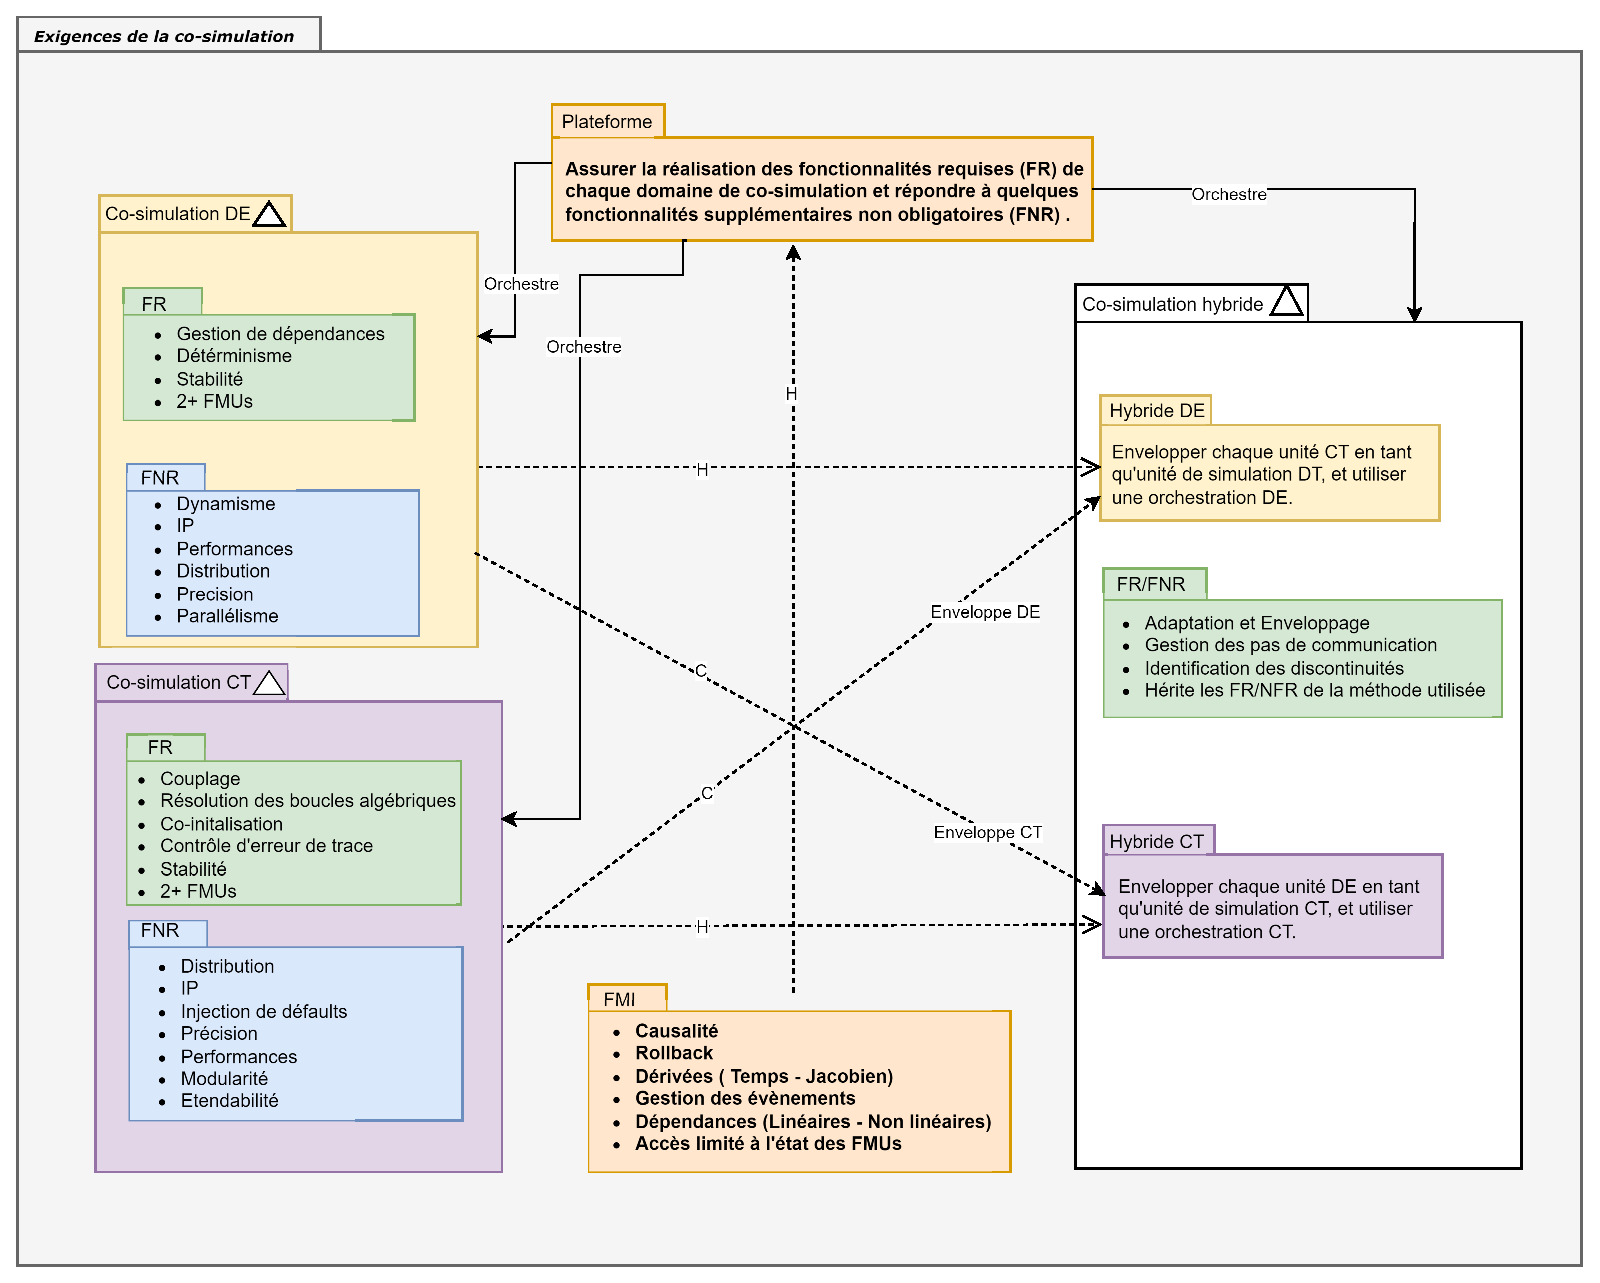
\includegraphics[width = 0.8\textwidth]{1.eps}
  \caption{Diagramme d'exigences internes de la co-simulation}
  \label{fig:1}
\end{figure}

La figure \ref{fig:1} offre une classification de la co-simulation, mettant en lumière les différentes propriétés requises ou optionnelles (FR/NFR) offertes par les divers intervenants de ce processus. Elle illustre les relations entre ces entités, telles que la liaison d'hérédité entre la plateforme et le standard FMI, offrant ainsi une vision holistique des interactions dans le domaine de la co-simulation.

D'autre part, la figure \ref{fig:2} dépeint d'une manière fonctionnelle les exigences décrites dans la figure \ref{fig:1}. En fournissant une représentation graphique du cheminement des exigences à travers les différentes entités de la co-simulation, cette figure offre une vue détaillée de la dynamique fonctionnelle de ce processus complexe.

\begin{figure}[hbt!]
  \centering
  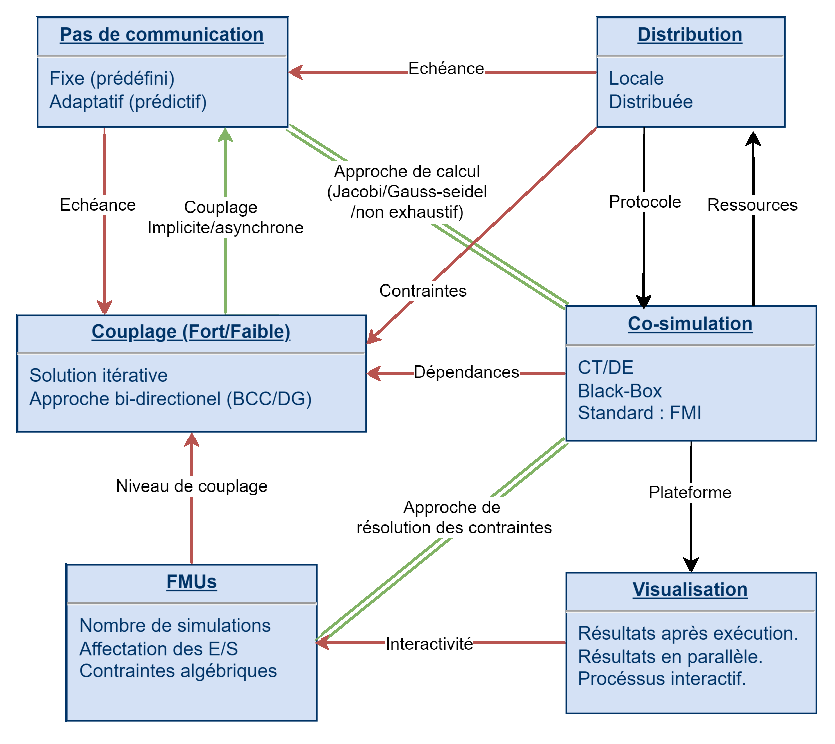
\includegraphics[width = 0.8\textwidth]{Diagramme-2.eps}
  \caption{Diagramme d'exigences fonctionnelles de la co-simulation}
  \label{fig:2}
\end{figure}


\section{Conclusion et perspectives}
Ce chapitre met en lumière les défis intrigants du domaine de la co-simulation. L'analyse commence par explorer séparément les deux principales approches : la co-simulation basée sur le temps continu et celle sur les événements discrets, avant d'examiner les difficultés associées à leur intégration. Une taxonomie basée sur des principes ontologiques et structurée en deux niveaux est ensuite introduite. La figure \ref{fig:1} illustre les interactions et les rôles des différentes entités impliquées, offrant un aperçu complet des aspects clés du processus, et servant également de modèle conceptuel pour le développement d'outils de co-simulation. Enfin, la figure \ref{fig:2} détaille les exigences de base et les approches correspondantes pour chaque entité, enrichissant ainsi notre compréhension de la structure fonctionnelle du sujet.

Au cours de cette étude, on a passé en revue plusieurs plateformes de co-simulation majeures, telles que Maestro2 \cite{b13}, OMSimulator\cite{b14} et Daccosim ng \cite{b15}. Une analyse comparative de ces plateformes, basée sur les fonctionnalités clés identifiées dans cette étude, fera l'objet du prochain chapitre.

